%\documentclass{sig-alternate-10pt}
\documentclass[10pt, two column]{article}

\usepackage{fullpage}
\usepackage{algorithmic}
\usepackage{algorithm}
\usepackage{hyperref}
\usepackage{cite}
\usepackage{url}
\usepackage{graphicx}
\usepackage{caption}
\usepackage{subcaption}
\usepackage{color}
\usepackage{comment}
\usepackage{multirow}
\usepackage{booktabs}
\usepackage{listings}
\newcommand{\XXX}[1]{\textcolor{blue}{\textit{XXX: {#1}}}}

\begin{document}

\title{FreEBS - A Distributed Virtual Block Device}

%\author{
%	\alignauthor Igor Canadi, Rebecca Lam, James Paton\\
%	\affaddr{University of Wisconsin-Madison}\\
%	\email{\{canadi,rjlam,jpaton\}@cs.wisc.edu}
%}

\author{
Igor Canadi\\
\texttt{canadi@cs.wisc.edu}
\and
Rebecca Lam\\
\texttt{rjlam@cs.wisc.edu}
\and
James Paton\\
\texttt{jpaton@cs.wisc.edu}
}
\date{}
\maketitle

\begin{abstract}
The primary goal of this project was to create a free, open-source 
implementation of Amazon EBS. We present FreEBS, a distributed virtual block
device that uses chained replication and log-based virtual disks with the 
goals of availability, durability, and reliability in mind. Our backing 
storage also provides the framework for snapshotting, one of
the main features of Amazon EBS that makes it more robust and resilient to
failure. 

We compare our system's performance to the performance of native I/O on a local disk. We find that, for random and mixed random-sequential workloads, FreEBS performs with much higher throughput than local, while for purely sequential workloads it performs much more poorly.

Finally, we argue that FreEBS points the way toward a viable commoditization of replicated block storage, exemplifying a novel model as compared to DRBD or SAN. This model has the potential to lower cost and increase performance.
\end{abstract}


\section{Introduction}
\label{sec:intro}
FreEBS is a distributed virtual block device that utilizes replication and 
log-based storage to provide reliability and durability. The major 
goal of FreEBS is to create a free and open version of Amazon Elastic Block 
Store (EBS)\cite{amazonEBS}, a virtual mountable block device used by EC2 
instances. Many implementation details about EBS have not been publicized,
but many speculate that EBS is based on 
DRBD\textsuperscript{\textregistered}\cite{drbd}. 

There are two main features that are publicly known about Amazon EBS --- 
replication and snapshots. EBS mirrors volume data across different 
servers within the same Availability Zone. This provides some increased 
reliability over a single disk, but EBS further adds durability using 
snapshots. Snapshots are 
customizable incremental backups stored on Amazon S3. Each snapshot only 
saves the blocks that have been modified since the last snapshot. For each
snapshot there is a table of contents that maps each EBS volume block to 
the valid corresponding block in S3. When a snapshot is deleted, only 
blocks that are not pointed to by any other snapshot are removed from S3. 
Because snapshots only keep track of modified blocks, they take less 
time to perform than a full-volume backup, and require less space to store. 
The frequency at which they are performed determines the durability of 
the volume in the case that the EBS volume fails. \cite{amazonEBS} 

Due to the lack of concrete, detailed information about Amazon EBS, we 
draw many of our ideas about how EBS is implemented from Distributed Replicated 
Block Device\textsuperscript{\textregistered} (DRBD)\cite{drbd}, an open source 
virtual RAID-1 block device. We discuss DRBD\textsuperscript{\textregistered}
in more detail in Section~\ref{sec:related}.

Given what we know of EBS and DRBD, FreEBS seeks to provide the below:

\begin{description}
    \item[Availability]{The system should continue to operate with a certain
            number of replica failures.}
    \item[Durability]{In the case of a failure, the most recent data should
            still exist on the volume.}
    \item[Reliability]{The system should operate as expected and behave
            deterministically.}
    \item[Snapshots]{Our backing file should support snapshots and incremental backups}
\end{description}

We address these goals by using replica servers that coordinate using a
userspace process on each machine. These replicas propagate writes and 
perform synchronization. They also interact with a log-structured virtual 
disk that provides checkpointing, mechanism for recovery, and the 
framework for snapshotting. 

\XXX{Talk briefly about results here?}

The rest of the paper is organized as follows. In Section~\ref{sec:related}
we discuss related work, and in Section~\ref{sec:design} we explain the 
overall design of the system. We go into more detail about our system in 
Section~\ref{sec:implementation}. Finally, we evaluate our design and draw
appropriate conclusions in Section~\ref{sec:evaluation} and 
Section~\ref{sec:conc}, respectively.


\section{Related Work}
\label{sec:related}
We drew many of our ideas about EBS on past 
work, especially DRBD\textsuperscript{\textregistered}. Here we 
discuss related network and cloud storage systems and compare our work to them.

\subsection{DRBD}
\label{sec:drbd}
DRBD\textsuperscript{\textregistered} is a virtual RAID-1 block storage 
device consisting of two shared-nothing nodes that form a highly available
\emph{cluster}. The DRBD\textsuperscript{\textregistered} interface is 
implemented as a kernel module that can be mounted like a normal block 
device. Since it is an open-source project, many aspects of its 
implementation are available; however, in this section we focus on the
details of replication and synchronization.

\subsubsection{Replication}
DRBD\textsuperscript{\textregistered} uses a RAID-1 method of replication, 
meaning there are two nodes in a basic DRBD\textsuperscript{\textregistered} 
cluster --- one \emph{primary} and one \emph{secondary} --- that each
contain typical Linux kernel components\cite{drbd, drbd_manual}. The 
primary node 
services all reads and writes, and the secondary node fully mirrors the 
primary node by propagation of writes across the network. If the primary 
node fails, then service migrates to the secondary node. There are two 
main modes for replication --- fully synchronous and asynchronous. 
The former means that the primary node reports a completed write only after 
the write has been committed to both nodes in the cluster. The latter means 
that each node reports a successful write as soon as the data is written to 
its local disk. 

FreEBS uses a technique similar to the asynchronous mode of replication;
we utilize a primary replica that services reads and propagates write 
requests. However, FreEBS waits for a majority of replicas to respond with a
successful write completion. Our system also offers much more flexibility in 
terms of the number of configurable replicas. For instance, 
DRBD\textsuperscript{\textregistered} must use 
stacked DRBD volumes in order to create more than two replicas, which can 
get cumbersome as we add more replicas.

\subsubsection{Synchronization} 
DRBD\textsuperscript{\textregistered} offers 
variable-rate and fixed-rate synchronization \cite{drbd_manual}.
For the first method, DRBD\textsuperscript{\textregistered} selects a 
synchronization rate
based on the network bandwidth. For the fixed-rate case, synchronization is
performed periodically at some constant time interval. Synchronization 
can be made more efficient by using checksums to identify blocks that have 
changed since the last synchronization. This eliminates the need to 
synchronize blocks that were overwritten with identical contents. Changes
are tracked using the activity log (AL) that records \emph{hot extents}, 
the blocks that have been modified between synchronization points. The 
activity log uses a quick-sync bitmap to keep track of modified blocks.

FreEBS uses a fixed-rate synchronization scheme that allows nodes to request 
all writes since a particular version. This is done by backward traversal 
through our log-based backing file until the requested version is found, 
eliminating the need to have a separate activity log.

%\emph{Should we include the DRBD figure here?}

\subsection{Cloud Storage}
Rackspace Cloud Block Storage (CBS) and HP Cloud Block Storage provide 
persistent storage for their cloud instances\cite{rackspace, hp}. Both also 
support snapshots. However, unlike EBS snapshots, Rackspace CBS snapshots
contain the 
full directory structure of a volume. Both HP CBS and Rackspace CBS are 
built on the OpenStack storage platform. Another commercially available 
cloud block storage is Zadara\texttrademark Virtual Private Storage 
Arrays\cite{zadara}, which is a cloud-based NAS service that uses iSCSI 
and NFS protocols.  

\subsection{Network Block Level Storage Systems}
There is a fair amount of work on the subject of network block level storage.
For instance, in 1996 Lee and Thekkath published a paper on Petal, a 
distributed virtual disk system\cite{lee1996petal}. In this system, a cluster
of servers manage a shared pool of physical disks and present the client 
with a virtual disk. Virtual disks are globally accessible to all
Petal clients, not one-to-one like FreEBS. Petal handles failure by 
chain-replicating blocks with one neighboring server. If one disk goes down,
then the server with the replica block will serve the request. 

In \cite{dabek2001wide} Dabek et al. discuss Cooperative File System (CFS), 
a peer-to-peer read-only block storage system with robustness and 
scalability in mind. CFS uses a distributed hash table to map blocks to a CFS
server and utilizes block-level replication to increase reliability. 
Block replicas exist on the subsequent $k$ servers based on the corresponding
hash value for that block; thus, the next server in the hash takes up 
responsibility for serving that block.  

Conversely, Quinlan and Dorward present Venti, a network storage system that
uses a write-once only policy for archival data\cite{quinlan2002venti}. Venti
is a userspace daemon that performs block level reads and permanent writes. 
Venti provides reliability and recovery by relying on RAID-5 disk arrays 
rather than mirroring.  

The main difference between these works and FreEBS is that they are built 
for a shared virtual disk system and thus consider scalability and load
balancing. FreEBS volumes, by contrast, only support being attached to one 
machine at a time. FreEBS also utilizes a log-based backing file to keep
track of changes, whereas the above systems do not.


\section{Design}
\label{sec:design}
\begin{figure}[b!]
    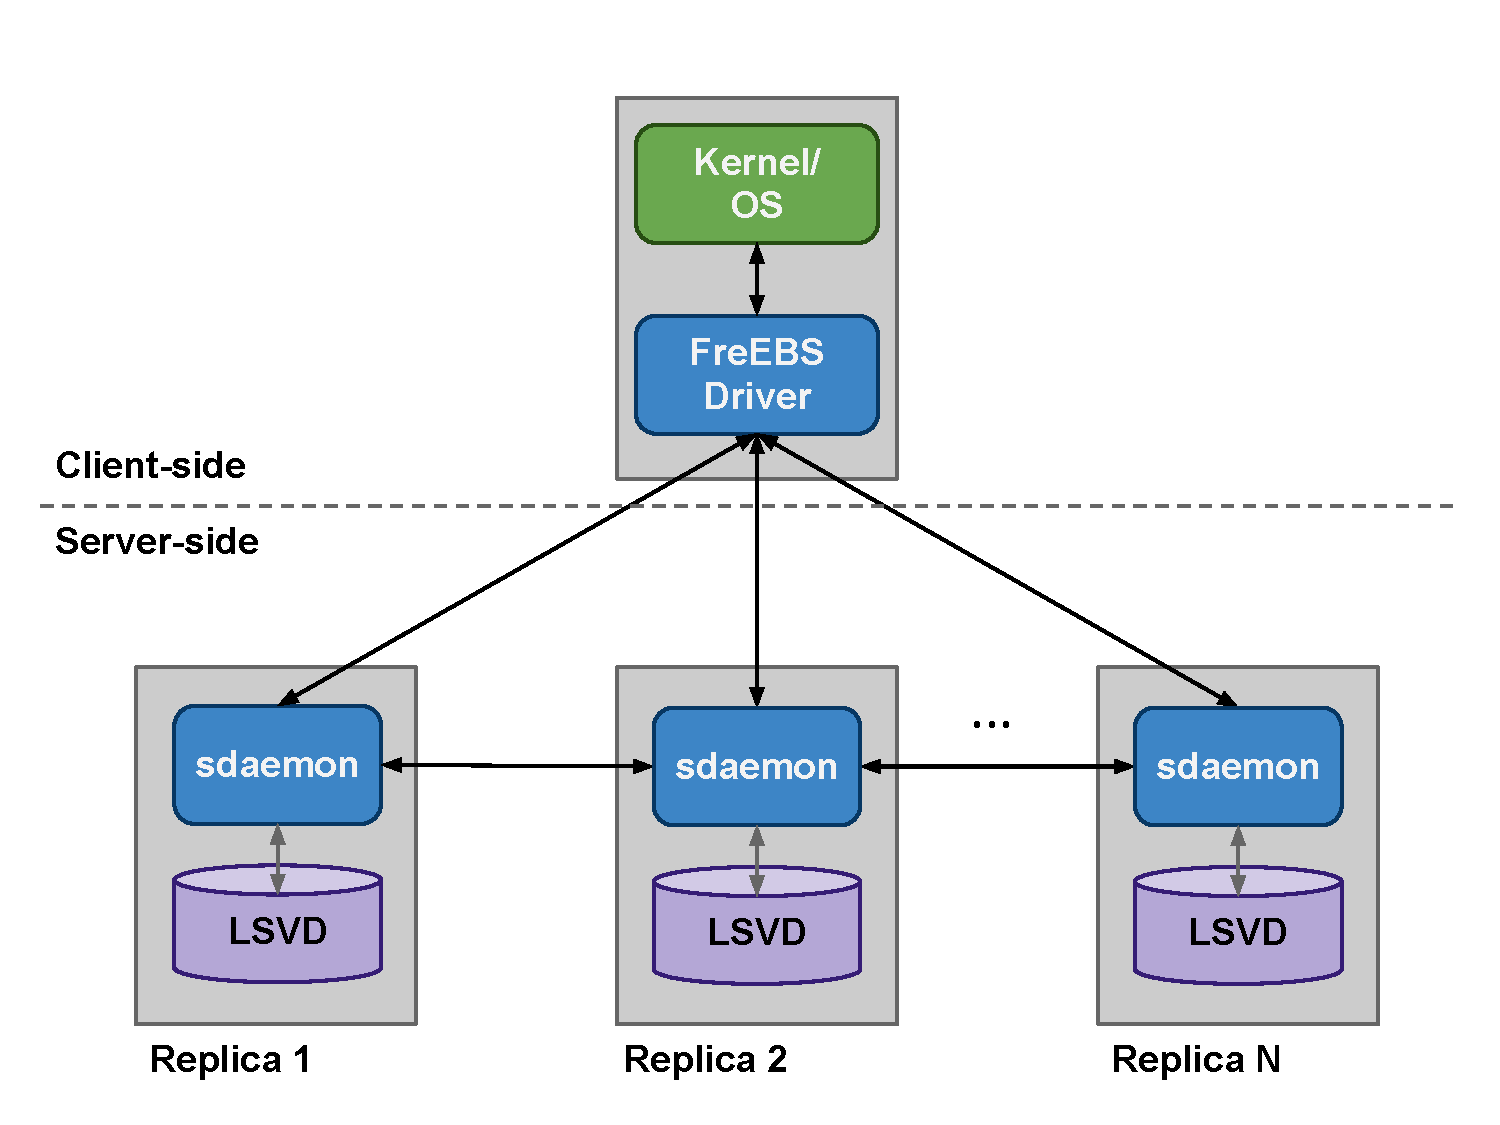
\includegraphics[width=0.45\textwidth]{./figures/systemarch.pdf}    
    \caption{The system architecture for FreEBS. A driver on the client 
            machine communicates with processes on the replicas on server 
            machines to read and write data.}
    \label{fig:architecture}
\end{figure}


FreEBS is a virtual block device backed by replication and log-structured
virtual disks for high reliability and availability. For all intents and 
purposes, the FreEBS storage system appears to the kernel as a normal block
device and thus reads and writes are issued to FreEBS without knowledge of 
its internals. The architecture of FreEBS is depicted in 
Figure~\ref{fig:architecture}. The most important component in
the system is the \emph{driver}, which is a kernel module that implements
kernel block device interface and exports a block device that can be mounted
on a system. The kernel forwards all device's read and write requests to the
driver. The driver forwards the requests appropriately to the 
\emph{replicas}. Our current configuration uses three replicas, but our 
design is flexible enough that we can arbitrarily add more replicas. We 
discuss replication in more detail in Section~\ref{sec:replication}.

Replicas are essentially server machines that communicate with each other 
and the driver across the network using a custom TCP protocol. Each replica 
runs a userspace process called \texttt{sdaemon} that is in 
charge of propagating write requests and synchronizing replicas. It is also
responsible for interfacing with its private copy of the underlying storage 
that actually holds the device data, \emph{Log Structured Virtual Disk}
(LSVD). LSVD is backed by a file on the server file system that uses a 
dynamically growing file format. It provides checkpointing and versioning 
for high data integrity. LSVD borrows ideas from Log Structured File System \cite{lfs}. A more in-depth discussion about LSVD is in Section~\ref{sec:lsvd}.

\section{Implementation}
\label{sec:implementation}
\subsection{Reads and Writes}
\label{sec:readwrite}
There are two operations that are issued by the driver --- read and write.
The driver keeps track of the most recent version for each replica in a list.
This structure is updated on a write and used to decide which replica to 
request a read from.

Figure~\ref{fig:write} shows the message flow on a write request. Notice
that we utilize chained replication, where the closer the replica is to the 
head of the chain the more more up-to-date it is. The choice for this chained
scheme is to reduce the network load to the driver. Thus, when 
the driver sends a write request, \texttt{sdaemon} issues the write to its 
local LSVD copy and then propagates the request to the next replica in the 
chain. After writing to its own LSVD, each replica sends back a response to
the driver with a status and its current version number. The driver then 
updates its replica list with the version in the sent response. If a majority
of replicas responds to the driver with a SUCCESS message, then the driver 
reports a success back to the kernel. Otherwise, it will report a failure. 

In contrast, a read only needs one replica to respond for a success. In 
Figure~\ref{fig:read} we observe that when the driver issues a read request 
it issues the request to the replica with the most recent version. Typically 
this is the primary replica. If the replica responds with a SUCCESS, then 
the driver serves the request back to the kernel. Otherwise, it will issue 
the request to the next replica in the chain with the most recent version. I 
no replicas respond, then the driver reports a failure.

\begin{figure}[t]
    \begin{subfigure}{0.5\textwidth}
        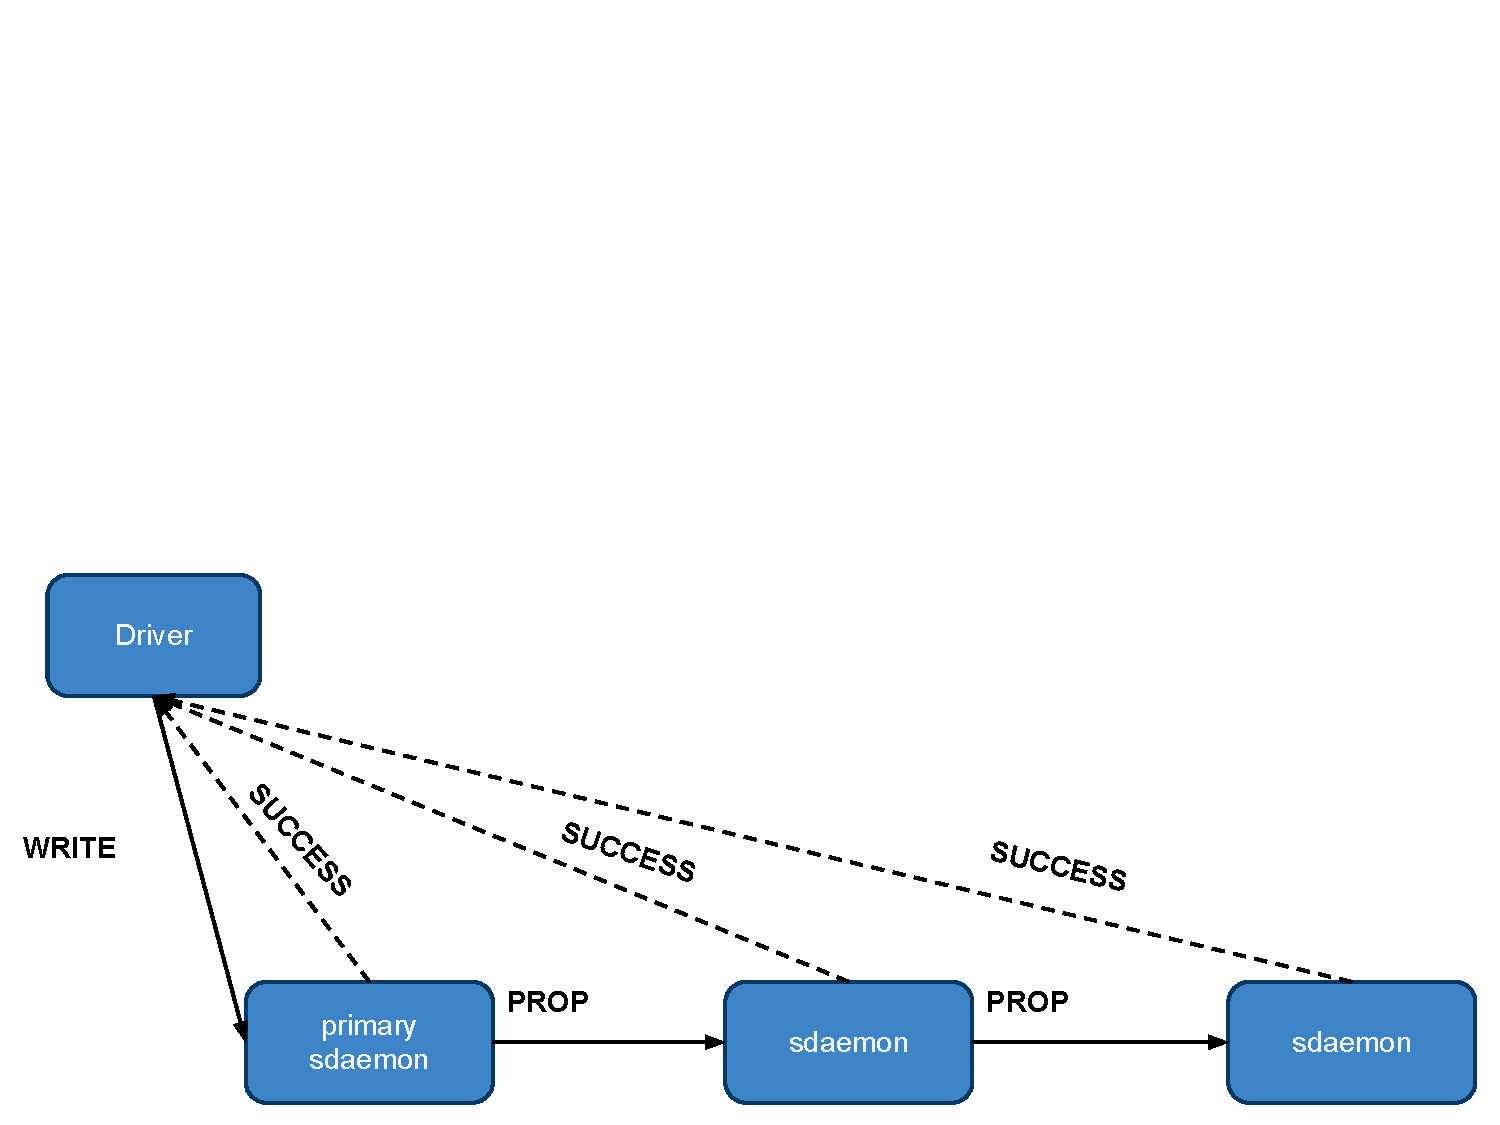
\includegraphics[width=\textwidth, trim=0 0 0 3.5in, clip]{./figures/write.pdf}
        \caption{The message flow for a write operation. A quorum of SUCCESS 
                 responses must be received for a successful write.}
        \label{fig:write}
    \end{subfigure}
    ~
    \begin{subfigure}{0.5\textwidth}
        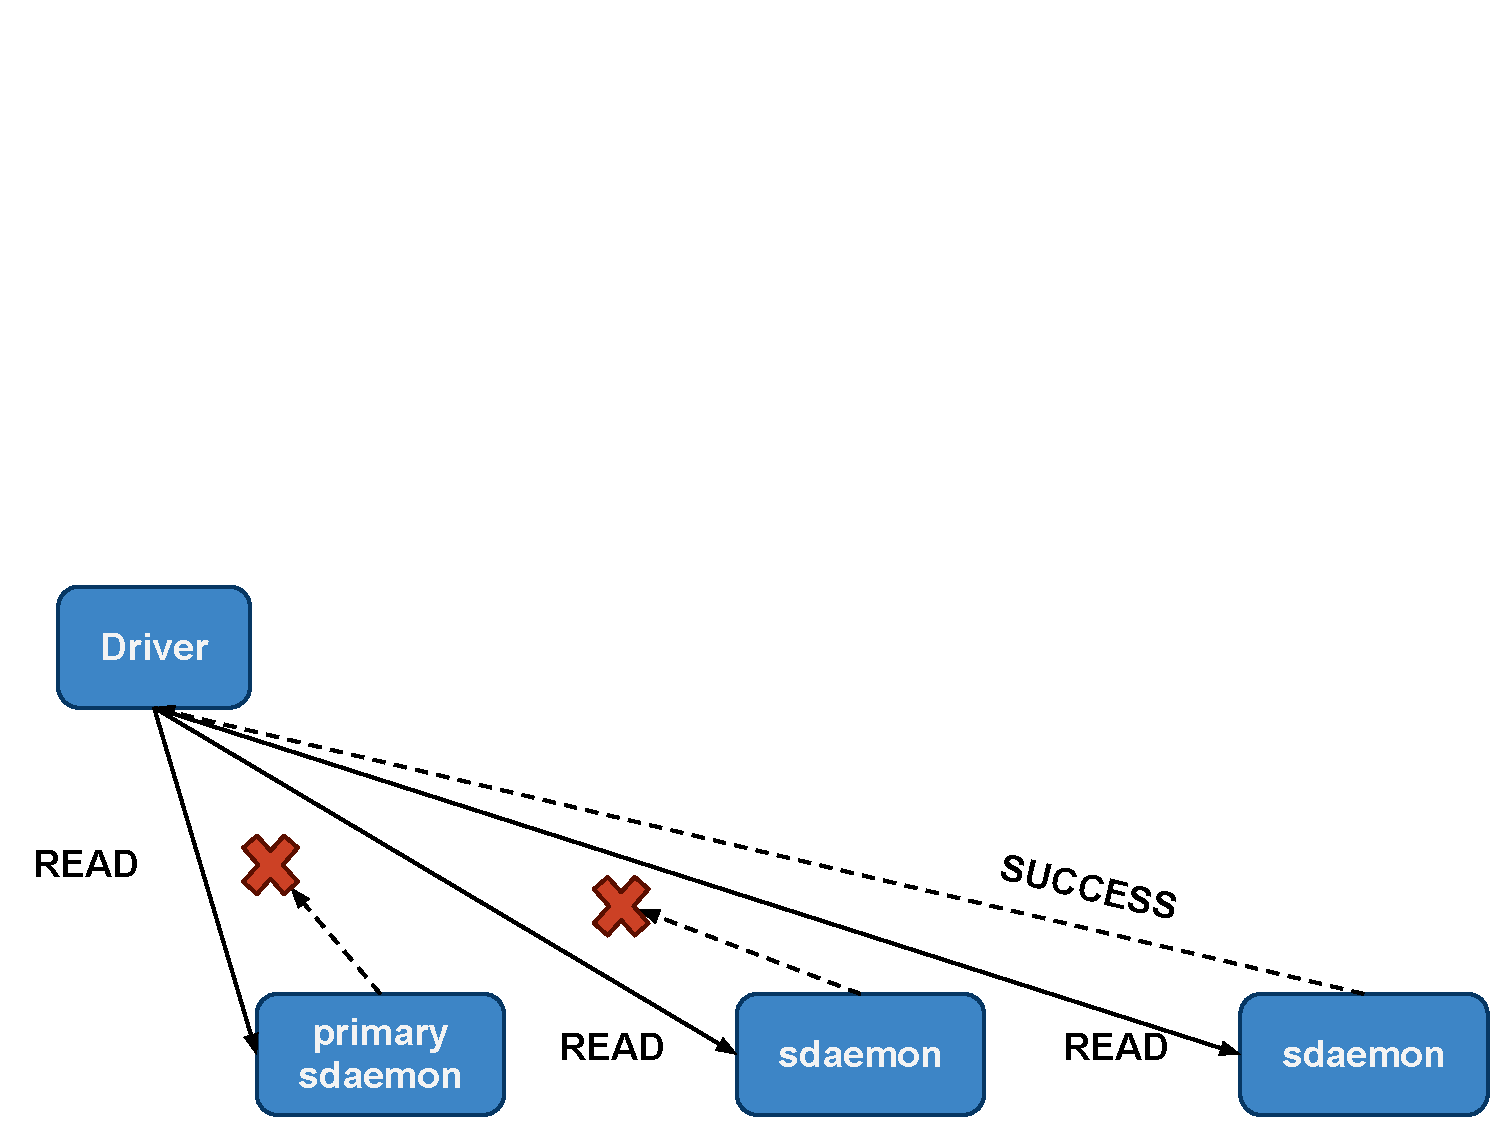
\includegraphics[width=\textwidth, trim=0 0 0 3.5in, clip]{./figures/read.pdf}
        \caption{The message flow for a read operation. A read request is 
            issued to the replica with the most recent version until a 
            SUCCESS is received or if no replicas with the most recent 
            version responds with SUCCESS.}
        \label{fig:read}
    \end{subfigure}
    \caption{Message flows for read and write operations}
\end{figure}

\subsection{Replication}
\label{sec:replication}
Replication is managed by \texttt{sdaemon} using write propagation and 
synchronization. Propagation was discussed in Section~\ref{sec:readwrite}. 
Synchronization is performed whenever a replica joins the chain and also 
periodically to keep replicas near the tail from becoming increasingly out 
of date. Figure~\ref{fig:sync} shows how replication is performed. As we see,
replica C sends a SYNC request with the version number of its local LSVD 
copy to the previous replica in the chain, replica B. Replica B then responds
with all the writes from C.version to B.version. Replica C then applies all 
the writes to its LSVD. After the synchronization operation, Replica C's 
LSVD version is equal to B's version. Similarly, replica B initiates the 
synchronization procedure with replica A.

To handle failure, a replica controller is used to inform the driver and 
neighboring replicas that a failure has occured. This controller keeps track 
of the liveliness of each replica by recording the elapsed time since the 
last heartbeat message, which is sent every $T$ seconds by each replica. After
$2T$ seconds the controller flags the replica as \emph{inactive} and after 
$4T$ seconds the replica is marked as failed. Upon failure, the controller 
informs the kernel and the neighboring replicas using update messages. Upon
receipt of the update messages, the two neighboring replicas connect to each
other. The latter replica sends a SYNC request, and then normal operation 
resumes. Meanwhile, the controller spins off a new \texttt{sdaemon} process
that is appended to the end of the chain. Note that currently the replica 
controller is not implemented.

\begin{figure}[t]
    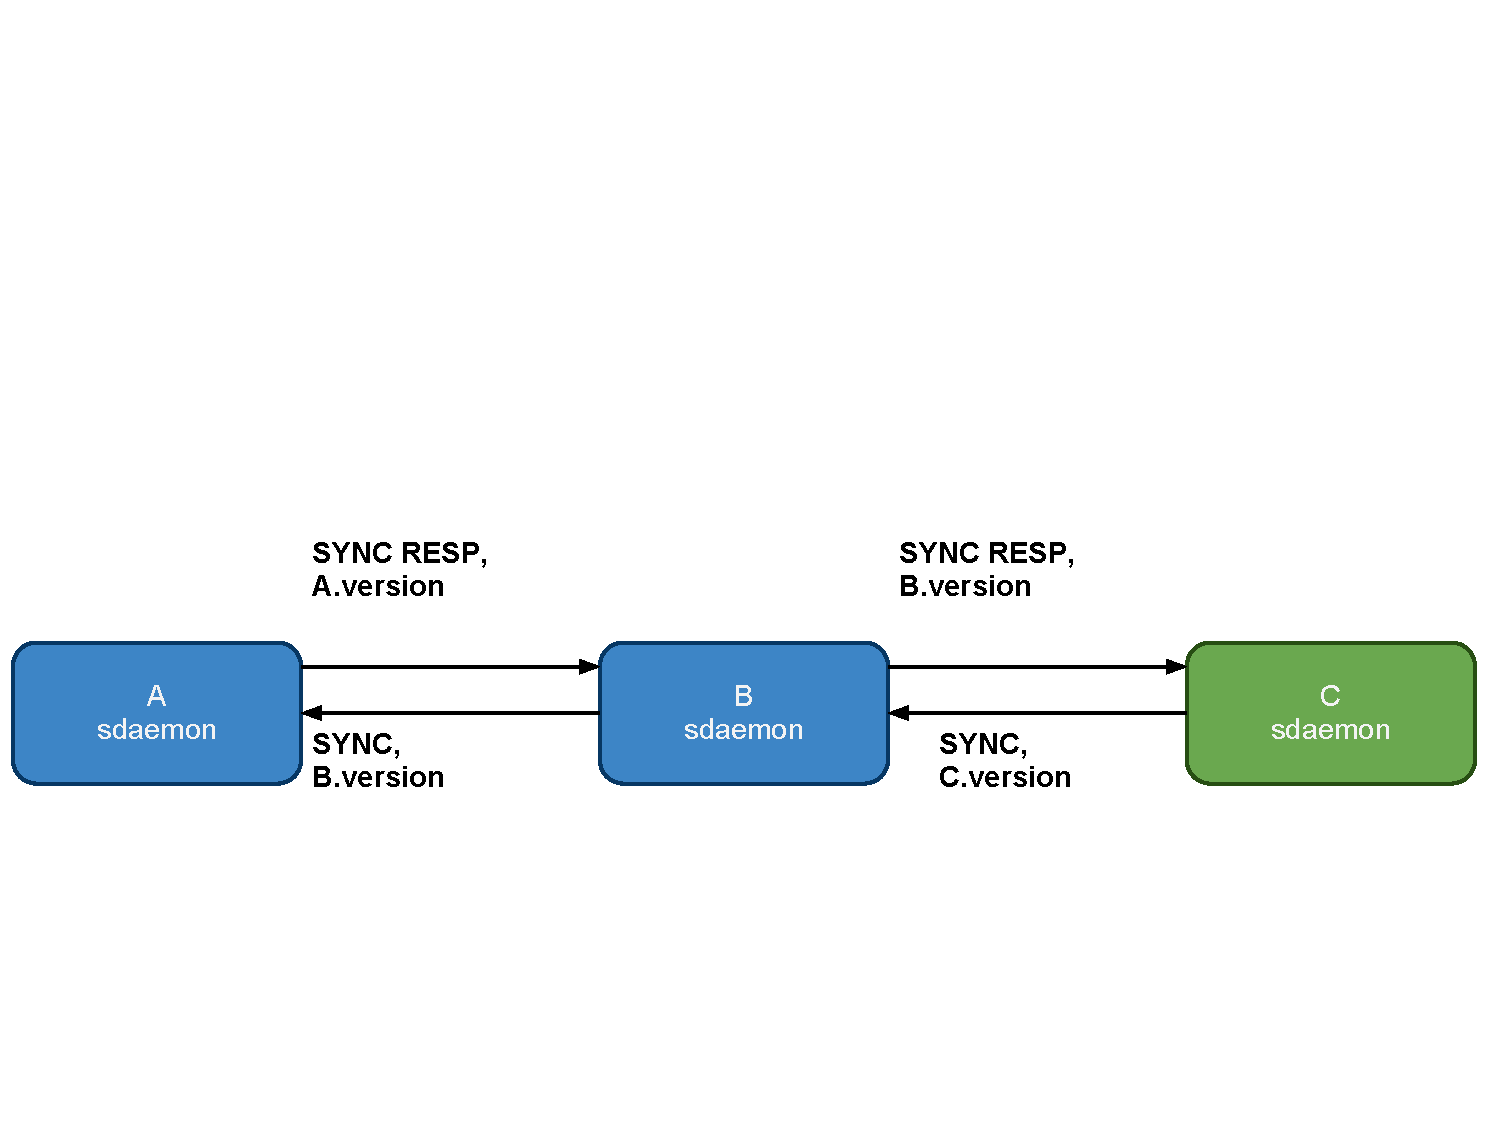
\includegraphics[width=0.45\textwidth, trim=0 2in 0 3in, clip]{./figures/sync.pdf}
    \caption{The message flow for a synchronization operation. Replica C 
            sends a SYNC request to its predecessor, which responds with all
            the writes since C's version.}
    \label{fig:sync}
\end{figure}

\subsection{Log Structured Virtual Disk}
\label{sec:lsvd}

When designing our file format to back virtual disk, we had few goals in mind. First, the file should be dynamically growing. If a disk was defined with $D$ bytes free space and user is using only $C$ bytes for his content, the backing file size should use $O(C)$ bytes. Second, we have to support versioning. We define version as update sequence number. Each update increments disk version by one. Update can consist of one or more sequential sectors on the disk and it's originating from Virtual Block Device in the kernel. To enable synchronization, storage daemon has to be aware of the current local disk version and has to be able to send arbitrary version updates to other replicas for synchronization. Third goals was consistency. If the local data has version $V$, it should include all updates with versions less than or equal to $V$ and none of the updates with versions bigger than $V$. Finally, our fourth goal was ability to easily support snapshots and incremental backups.

To address all these requirements, we developed Log Structured Virtual Disk (LSVD). When we receive updates, we just write them sequentially on a disk and increment version number by one. That way, we are dynamically growing. We also support versioning and are consistent, since we remember all updates together with their version numbers. When implementing the file format, we took special care to make sure that if we fail at any arbitrary point in time, the file is still consistent and can be recovered up to some recent version number. Finally, it is easy to support snapshoting and incremental backups. On snapshot operation, we just create new file and use old file as a base. New updates go to the new file and we can read old data from old, read-only base file. \XXX{Extend this?}

Figure \ref{fig:lsvd} shows the actual data layout in LSVD file. First few bytes define the superblock, which contains important metadata. Next, there are two checkpointing placeholders. After that, actual updates are layed out. Each update consists of data block and commit block. Data block can hold one or more sectors. Io our implementation, we use 4KB sector sizes. Commit block verifies integrity of the data block by storing its checksum. To be able to guarantee consistency, we need to have atomic version writes. If a commit block is not written to disk or checksum is invalid, we define the update as not committed.

\begin{figure}[h]
    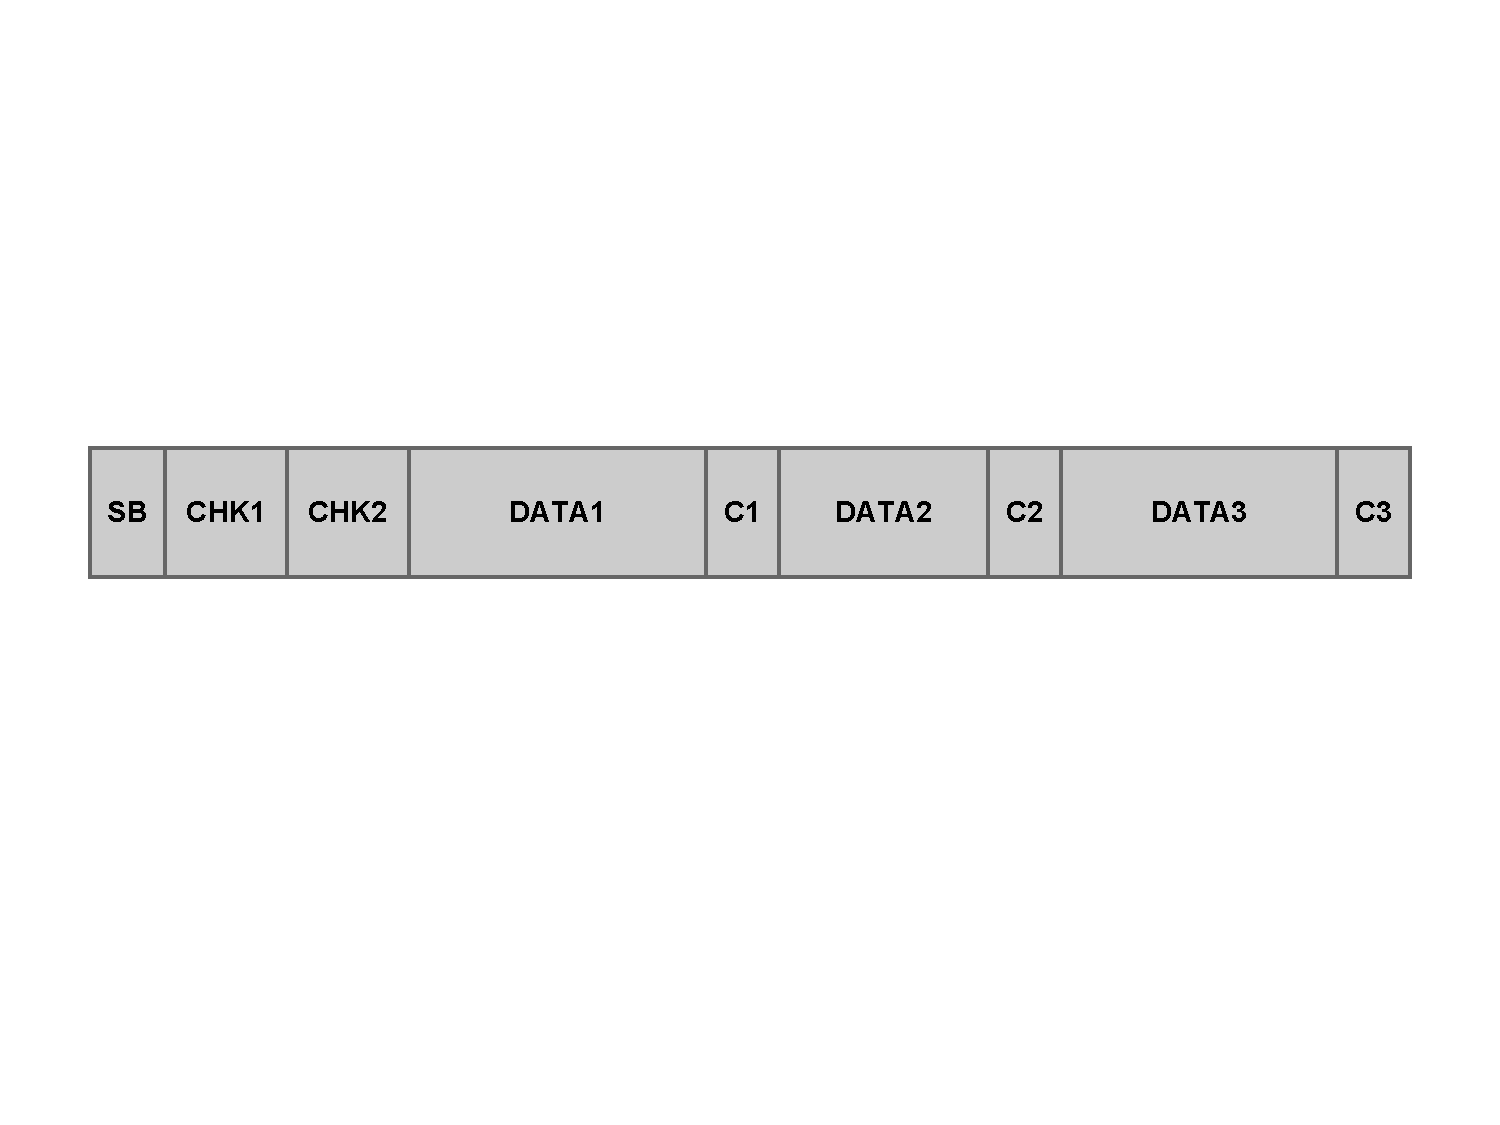
\includegraphics[width=0.45\textwidth]{./figures/lsvd.pdf}
    \caption{The LSVD file structure.}
    \label{fig:lsvd}
\end{figure}


On a write, we just append write to the end of the file with additional metadata. Therefore, on a read we need to be able to find requested sectors on the disk. For that, we keep in-memory \emph{sector to offset map}. It maps disk sectors to file offsets where the sector's data is stored. On every write, we easily update the map. When opening a disk after recovery, we are able to rebuild sector to offset map by reading all the updates from the beginning of time. That would, however, be very slow. To keep recovery time from growing linearly with time, we do \emph{checkpointing}. Every 60 seconds, we write the sector to offset map to disk into one of the checkpointing placeholders at the beginning of the file. We execute checkpointing writes slowly. That way, we do not slow down regular write or read operations, especially since checkpointing writes are random writes. Superblock keeps a pointer to an active checkpoint. After the checkpoint is fully written to one of the placeholders, we update the superblock and \texttt{fsync}. During recovery, checkpoint is loaded into memory and recovery continues from the point in time when checkpoint was started. That way, we limit recovery time and keep it from not growing linearly with time.

The problem with storing data in log structured format is garbage collection. Even though a sector has been overwritten by newer data, we still keep an old version around. We can use it to our advantage and provide a feature that enables users to recover the disk state from arbitrary point in time. However, we decided to implement garbage collection with a goal of reclaiming state from sectors that have been overwritten with newer data. To do this, we developed a separate \texttt{cleanup} function that reads in a LSVD file and creates a new file containing only up-to-date updates. The \texttt{cleanup} function reads in the file and reconstructs sector to offset map. It then starts at the beginning of the file and considers all updates on the disk. If any of the sectors contained in an update is up-to-date, the update is appended to the new file. If all of the sectors have been overwritten, the update is skipped. Since the LSVD file is consistent on a disk at any point in time, we can execute cleanup during live operation. Once the new file is constructed, it can be brought up to date with the replica synchronization protocol. After it has been brought up to date, we can transparently change the active to and delete the old file. We have not implemented the hot swap, though. We evaluated cleanup function on offline LSVD files. There are two drawback of this garbage collection approach. First, it has to read in and process the whole file, which is a slow operation. Second, it requires enough free space on the current drive to store the new file. However, if we store $O(n)$ files on the disk and run cleanup on them in round robin fashion, we need free space for only $O(1)$ disks.



\section{Evaluation}
\label{sec:evaluation}
\subsection{File System Benchmarks}


\subsection{Checkpointing evaluation}
\begin{figure}
  \centering
   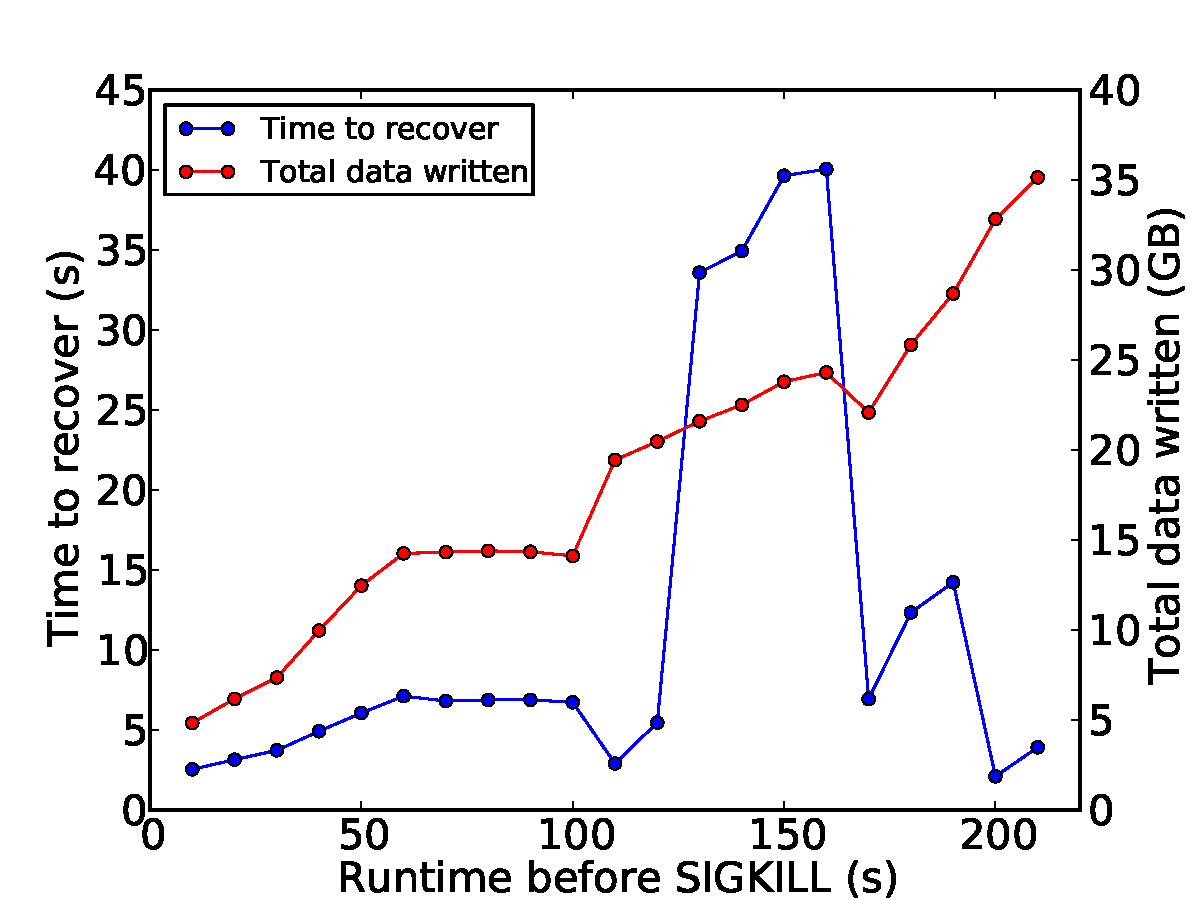
\includegraphics[width=3.5in]{figures/checkpointing.pdf}
   \caption{TODO}
   \label{fig:checkpointing}
\end{figure}

\section{Conclusion}
\label{sec:conc}
Presently, replicated block stores seem to be dominated by either DRBD-style or commercial NAS solutions. DRBD has the disadvantage that it is somewhat inflexible: it only allows two replicas (without stacking) and lacks dynamically resizing disk images. Further, DRBD puts all of its logic into a Linux kernel driver, making it more difficult to port to different systems. Commercial NAS solutions have the disadvantage of expense and opacity.

FreEBS shows that one can profitably move most of the replication logic into userspace programs. When the kernel driver becomes much simpler, it becomes more portable and reliable. Further, the replica managers themselves are more portable and maintainable. FreEBS is also a strong step in the direction of commoditizing replicated block storage for cloud computing since it enables such technology to be run on commodity hardware.

\bibliographystyle{plain}
\bibliography{biblio}

\end{document}



